\index{general}{Griffith-Murrell}
\begin{flushright} {\tiny {\color{gray} griffith\_murrell.tex}} \end{flushright}
%~~~~~~~~~~~~~~~~~~~~~~~~~~~~~~~~~~~~~~~~~~~~~~~~~~~~~~~~~~~~~~~~~~~~~~~~~~~~~~~~~~~~~~~~~~~~~~~~~~

The Griffith-Murrell yield criterion is not often used.
Noticeable exceptions are \textcite{brau94} (1994), \textcite{brbe95} (1995), \textcite{babr97} (1997).
In \textcite{brau94} (1994) we read:
\begin{displayquote}
Extending the work of Griffith (1921) to three dimensional stress distributions, 
Murrell (1963) suggested the following criterion for rock failure expressed 
in terms of the principal stresses:
\[
(\sigma_1-\sigma_2)^2 + (\sigma_2-\sigma_3)^2 + (\sigma_3-\sigma_1)^2
+
24T_0 (\sigma_1+\sigma_2+\sigma_3)=0
\]
where $T_0$ is a material property called the tensile strength. In principal stress space, 
this criterion is represented by a paraboloid of revolution around the pressure (or hydrostatic) axis.
\end{displayquote}

\noindent Using the definition of ${\III}_2({\bm \tau})$ of Eq.~\eqref{eq:I2s123} and ${\III}_1({\bm \sigma})$ of 
Eq.~\eqref{eq:I1s123}, it also writes:
\[
6 \left[\underbrace{\frac16 (\sigma_1-\sigma_2)^2 + (\sigma_2-\sigma_3)^2 + (\sigma_3-\sigma_1)^2}_{\III_2(\bm \tau)} \right]
+
24 T_0 \underbrace{(\sigma_1+\sigma_2+\sigma_3)}_{\III_1(\bm\sigma)}=0
\]
or,
\[
{\III}_2({\bm \tau}) + 4 T_0 \III_1(\bm\sigma) =0
\]
which is the formulation found in \textcite{brbe95} (1995). Furthermore the authors add:
\begin{displayquote}
A material that obeys this failure criterion can
be interpreted to be a frictional material in which the
strength increases in proportion to the square root of the
pressure. The failure envelope, $\FFF=0$, is a paraboloid
of revolution about the pressure axis in principal stress space
in contrast to the prismatic cone of the Mohr-Coulomb criterion.
\end{displayquote}
It is also worth mentioning that the authors explain the numerical methods
(FEM, plasticity implementation, solver) in the appendix.

Note that \textcite{hanl00} (2000) use an identical formulation, although 
the authors use the lithostatic pressure instead of the full pressure. 
They also use a tensile 
strength parameter $T_0^e$ and a compressive strength parameter $T_0^c$, both around a few tens 
of MPas. They refer to the book by Jaeger \& Cook (1979) when presenting the Griffith criterion. 
We find there (new edition of 2007, chapter 10.9) the same equation 
but with a minus sign:

\[
(\sigma_1-\sigma_2)^2 + (\sigma_2-\sigma_3)^2 + (\sigma_3-\sigma_1)^2
=
24T_0 (\sigma_1+\sigma_2+\sigma_3)
\]

It is not easy to find numerical values for the $T_0$ value, but in \textcite{babr97} (1997) we find  
in Table 2: $T_0=10^7~\si{\pascal}$ and in \textcite{hanl00} we find this great useful table:
\begin{center}
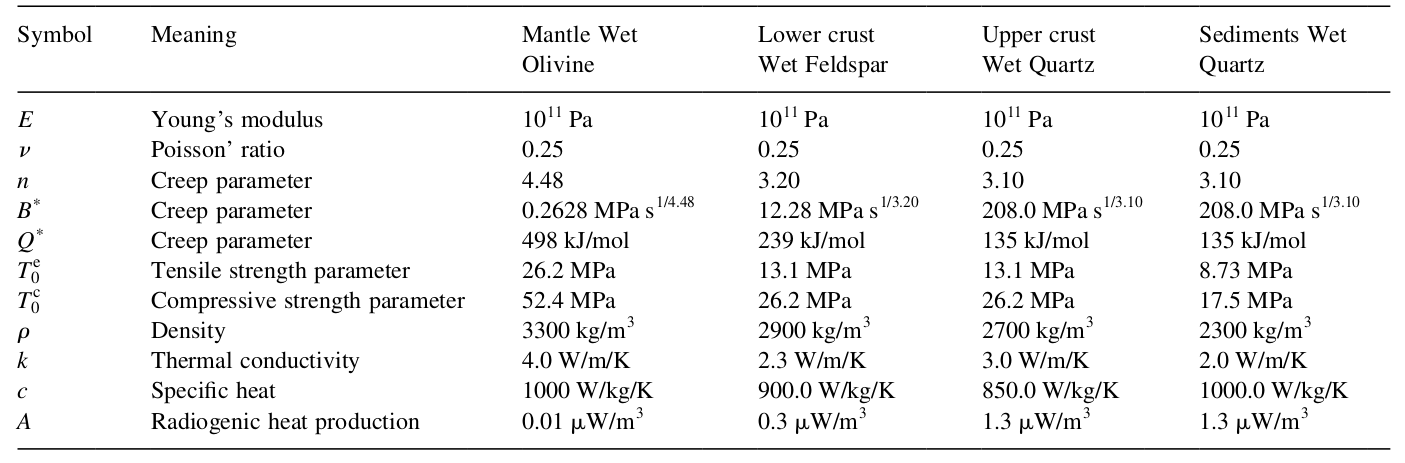
\includegraphics[width=13cm]{images/griffith_murrell/hanl00}
\end{center}




